\documentclass[a4paper,12pt]{article}
\usepackage{times}
\usepackage{setspace}
\usepackage{SIunits}
\usepackage{indentfirst}
\usepackage{graphicx}
\usepackage[top=25.4mm,bottom=25.4mm,left=31.8mm,right=31.8mm]{geometry}
\usepackage{fancyhdr}
\usepackage{amsmath}

\pagestyle{fancy}
\chead{\bfseries Center for Earth System Science}


\title{\textbf{GC Homework}}
\date{}
\author{Qifeng Qian, Bosong Zhang}

\begin{document}

\maketitle
\thispagestyle{fancy}
\chead{\bfseries Center for Earth System Science}

\begin{figure}[ht]
\centering
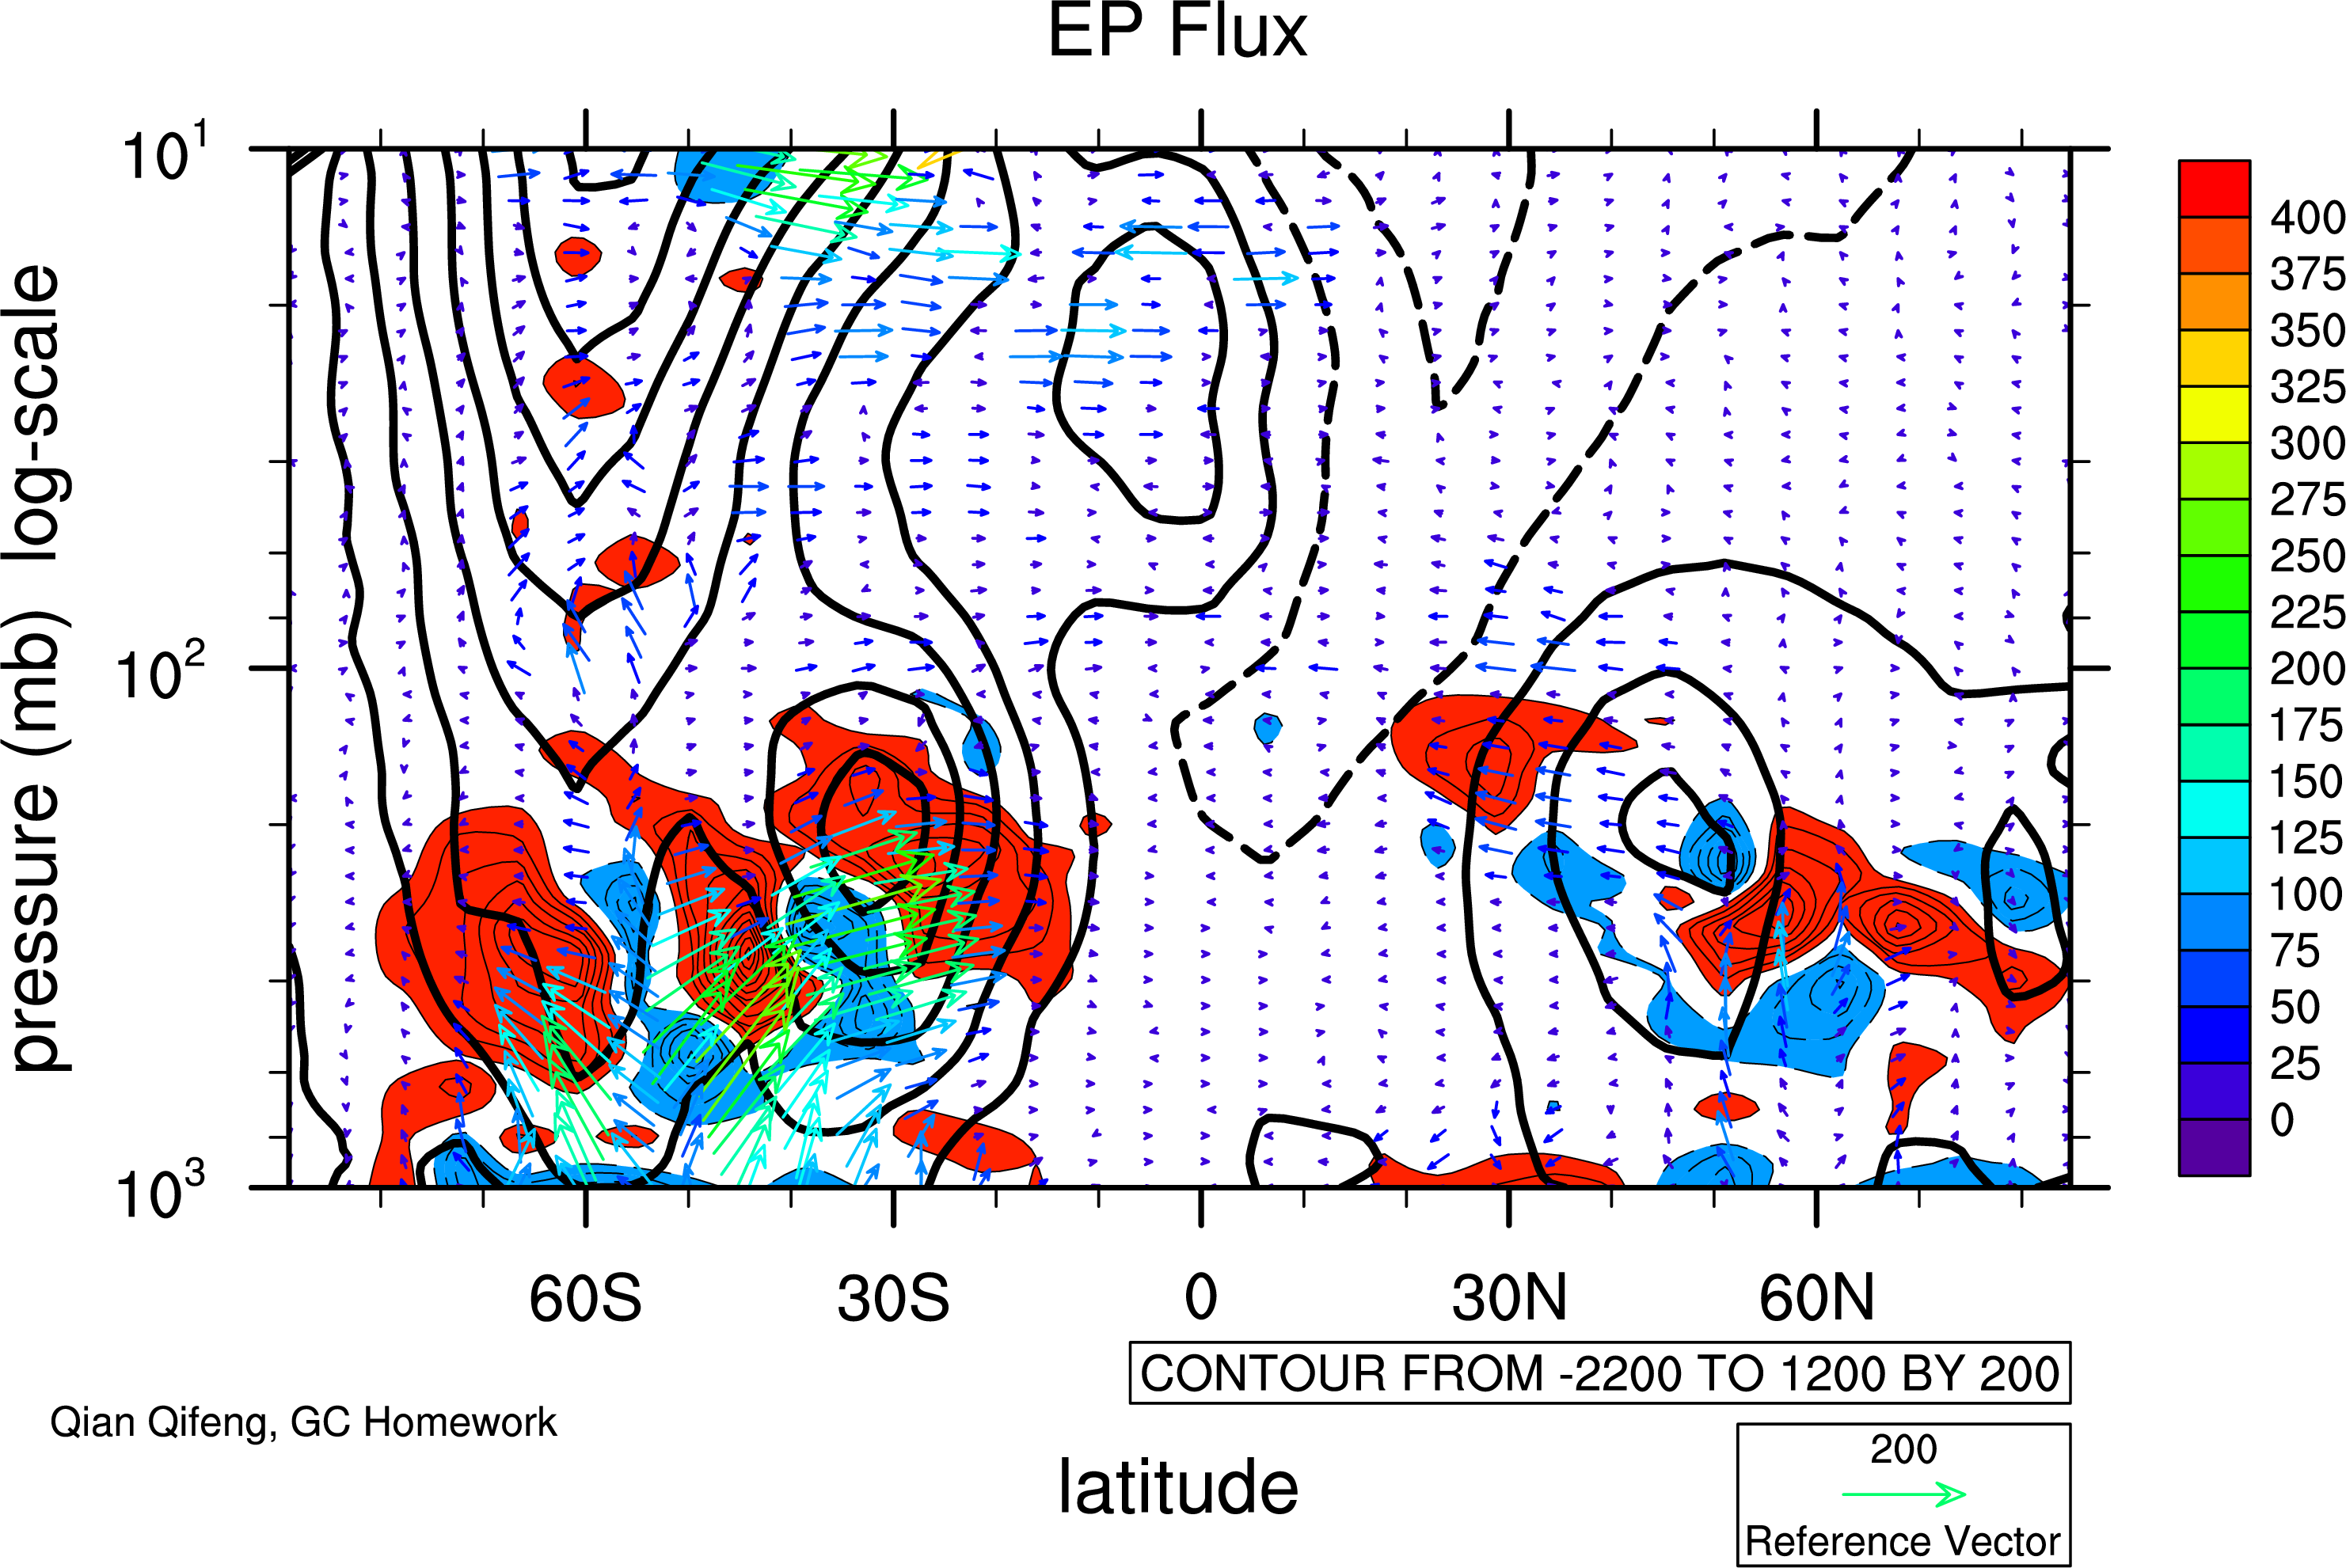
\includegraphics[height=9.52cm,width=14.82cm]{./EP.png}
\caption{This figure is about EP flux ploted with log pressure vertical coordinate. The vector is EP flux, and its color is the magnitude. The thick contour is zonal mean zonal wind. The thin solid line with red means the convergence of EP flux and the dashed line with blue means the divergence.}
\end{figure}

\parindent=15pt
\doublespacing
Previous studies show that EP flux has some important properties. The divergence of EP flux is related to the northward qasi-geostrophic potential-vorticity flux. What's more, the divergence of EP flux is also related to a so called density of "EP wave activity". EP flux also relate to the residual circulation.\newline
\centerline{$\nabla\cdot F=\overline{v'q'}$} \newline
\centerline{$\dfrac{\partial{A}}{\partial{t}}+\nabla\cdot{F}=0$}\newline
\centerline{$\dfrac{\partial{\bar{u}}}{\partial{t}}-f\bar{v^*}=\nabla\cdot{F}$}\par

We can see that in the southern hemisphere, EP flux converge near the troposphere subtropical jet. As a result, subtropical jet will be weaken according to the third equation (right side of the equation is negative, leading to $\dfrac{\partial{u}}{\partial{t}}<0$ which means deceleration). In fact, EP flux can not cross over the jet vertically, it always turn direction near the jet. In the subtropical region, there is EP flux convergence zone in the lower level and divergence zone in the upper level in the troposphere. This pattern is related to barotropical decay according to Edmon (1980) which will decrease the jet stream. In fact, EP flux pattern actually relate to the baroclinic instability. The convergence region is extending equatorward along the tropopause. The equatorward flux is quite large and growth has ceased.\par

It is quite manifest that near 50\degree S the EP flux direction is opposite, lower is equatorward and higher is polarward. So the source of EP flux is near 50\degree S. In upper troposphere near 50\degree S there is also a EP flux source. This is probably associated with nonlinear interaction between transient and stationary waves. \par

In the northern hemisphere, it is summer. Wave activity is weaker in summer than winter. We can clearly see that EP flux is small in northern hemisphere relatively. There is a divergence of EP flux near the jet stream, so it will accelerate.\par

However, in higher latitude of stratosphere, EP flux can generate residual circulation. In this case, we have $\nabla\cdot{F}<0$ leading to $\bar{v^*}>0$. So, there is a southward residual circulation in the southern hemisphere in the stratosphere.

Here is another explanation with deep and shallow forces. \par

If the ratio of the Coriolis force to the divergence of EP flux is much less than 1, which means that wave forcing is much stronger than the effect of Earth rotation, the dominant effect of EP flux is to accelerate or decelerate the zonal wind. When the EP flux is divergence, the zonal wind will accelerate, while convergence decelerate the zonal wind. In the plot, there is a westerly core in 30\degree S and the transient divergence of EP flux is negative. So the westward wind will decrease in the near future.\par

The Coriolis parameter $f=2\Omega sin(lat)$ is proportional to the latitude. So in high latitude, Coriolis force becomes more important, which means wave forcing has much effect on the meridional circulation rather than the zonal wind. From the plot we can infer that to the south of 60\degree S there is a convergence center of EP flux. So it will sustain the poleward residual velocity.\par

Actually both of them contribute not only zonal wind acceleration but also meridional circulation. The key parameter $f_{0}/N$ is to differentiate their effects. When the ratio of meridional wave number $k_{y}$ to vertical wave number $k_{z}$ is much larger than $f_{0}/N$, it��s called deep forcing. And it��s shallow forcing when the ratio is much smaller than $f_{0}/N$. \par

Downward control effect to explain the poleward residual velocity in low latitude. The plot shows that a wave source in the troposphere propagates upwards, and then bifurcates to 2 flows with one poleward and the other equatorward. For the one go equatorward, according to the downward control, the vertical velocity at a given height is determined by the wave forcing above the height. The EP flux is mainly convergence in the stratosphere. So the residual vertical velocity is positive, which coincides with the B-D circulation.



\newpage
\singlespacing
\noindent; Draw EP Flux and its divergence or acceleration\newline
; QQF\newline
; 2014.12.22\newline
\newline
load "\$NCARG\_ROOT/lib/ncarg/nclscripts/csm/contributed.ncl"\newline
load "\$NCARG\_ROOT/lib/ncarg/nclscripts/csm/gsn\_code.ncl"\newline
load "\$NCARG\_ROOT/lib/ncarg/nclscripts/csm/gsn\_csm.ncl"\newline           
load "\$NCARG\_ROOT/lib/ncarg/nclscripts/csm/shea\_util.ncl"\newline 
\newline
datafile=addfile("20080710\_00Z\_T85LR\_ECMWF\_876601148.nc","r")\newline
\newline
u\_hybrid=datafile-\verb">"U\newline
v\_hybrid=datafile-\verb">"V\newline
t\_hybrid=datafile-\verb">"T\newline
PS=datafile-\verb">"PS      ;Pa\newline
P0=datafile-\verb">"P0      ;Pa\newline    
hyam=datafile-\verb">"hyam\newline
hybm=datafile-\verb">"hybm\newline
lat=datafile-\verb">"lat\newline
lon=datafile-\verb">"lon\newline
lev=datafile-\verb">"lev\newline
PHIS=datafile-\verb">"PHIS\newline
nlev=dimsizes(lev)\newline
nlat=dimsizes(lat)\newline
nlon=dimsizes(lon)\newline
\newline
p\_level=10\^{}fspan(0,3,61)\newline 
n\_plev=dimsizes(p\_level)\newline
intyp=3\newline
kxtrp=True\newline
tbot=t\_hybrid(:,nlev-1,:,:)\newline
\newline
sf=5\newline
\newline
varflag=1\newline
T=vinth2p\_ecmwf(t\_hybrid,hyam,hybm,p\_level,PS,intyp,P0/100.0,1,kxtrp,varflag,tbot,PHIS)\newline
varflg = 0\newline
U=vinth2p\_ecmwf(u\_hybrid,hyam,hybm,p\_level,PS,intyp,P0/100.0,1,kxtrp,varflag,tbot,PHIS)\newline
V=vinth2p\_ecmwf(v\_hybrid,hyam,hybm,p\_level,PS,intyp,P0/100.0,1,kxtrp,varflag,tbot,PHIS)\newline
\newline
R=287.0\newline
Cp=1.005*(10\^{}3)\newline
theta=T*(1000.0/conform(T,p\_level,1))\^{}(R/Cp)\newline
copy\_VarMeta(T,theta)\newline
\newline
theta\_zonal\_mean=dim\_avg\_n\_Wrap(theta,3)                        ;0 is time, 1 is level, 2 is lat, 3 is lon\newline
Theta\_p=center\_finite\_diff\_n(theta\_zonal\_mean,p\_level*100.0,False,0,1)\newline
copy\_VarMeta(theta\_zonal\_mean,Theta\_p)\newline
\newline
u\_zonal\_mean=dim\_avg\_n\_Wrap(U,3)\newline
v\_zonal\_mean=dim\_avg\_n\_Wrap(V,3)\newline
\newline
u\_zonal\_anomaly=dim\_rmvmean\_n\_Wrap(U,3)\newline
v\_zonal\_anomaly=dim\_rmvmean\_n\_Wrap(V,3)\newline
theta\_zonal\_anomaly=dim\_rmvmean\_n\_Wrap(theta,3)\newline
\newline
uv=u\_zonal\_anomaly*v\_zonal\_anomaly\newline
copy\_VarMeta(u\_zonal\_anomaly,uv)\newline
uv\_zonal\_mean=dim\_avg\_n\_Wrap(uv,3)\newline
\newline
vtheta=v\_zonal\_anomaly*theta\_zonal\_anomaly\newline
copy\_VarMeta(theta\_zonal\_anomaly,vtheta)\newline
vtheta\_zonal\_mean=dim\_avg\_n\_Wrap(vtheta,3)\newline
\newline
a=6.37122e06\newline
pi=3.14159265358979\newline
phi=lat*pi/180.0\newline
a\_cos\_phi=a*cos(phi)\newline
a\_sin\_phi=a*sin(phi)\newline
omega=7.2921e-5\newline
f=2.0*omega*sin(phi)\newline
\newline
latfac=a\_cos\_phi*cos(phi)\newline
\newline
F\_phi=-uv\_zonal\_mean*conform(uv\_zonal\_mean,latfac,2)\newline
copy\_VarMeta(uv\_zonal\_mean,F\_phi)\newline
F\_p=conform(vtheta\_zonal\_mean,f*a\_cos\_phi,2)*vtheta\_zonal\_mean/Theta\_p\newline
copy\_VarMeta(vtheta\_zonal\_mean,F\_p)\newline
\newline
EP\_div\_phi=center\_finite\_diff\_n(F\_phi,a\_sin\_phi,False,0,2)\newline
copy\_VarMeta(F\_phi,EP\_div\_phi)\newline
EP\_div\_p=center\_finite\_diff\_n(F\_p,p\_level*100.0,False,0,1)\newline
copy\_VarMeta(F\_p,EP\_div\_p)\newline
EP\_div=EP\_div\_phi+EP\_div\_p\newline
copy\_VarMeta(F\_p,EP\_div)\newline
\newline
dudt=86400.0*EP\_div/conform(EP\_div,a*cos(phi),2)\newline 
copy\_VarMeta(EP\_div,dudt)\newline
\newline
F\_p=F\_p*conform(F\_p,cos(phi),2)\newline   
F\_phi=F\_phi/a\newline
\newline
F\_p=F\_p/1.0e5\newline
F\_phi=F\_phi/pi\newline
\newline
rhofac=sqrt(1000.0/p\_level)\newline
F\_p=F\_p*conform(F\_p,rhofac,1)\newline
F\_phi=F\_phi*conform(F\_phi,rhofac,1)\newline
\newline
strat1 = new(n\_plev,float)\newline
strat1=1\newline
ind\_100=ind(p\_level.le.100)\newline
strat1(ind\_100)=sf\newline
stratmask=conform(F\_p,strat1,1)\newline
F\_p=F\_p*stratmask\newline
F\_phi=F\_phi*stratmask\newline
\newline
res\_vec\_int=True\newline
res\_vec\_int @gsnDraw=False        \newline       
res\_vec\_int @gsnFrame=False \newline
res\_vec\_int @gsnSpreadColors=True	\newline
res\_vec\_int @gsnLeftString=""\newline
res\_vec\_int @gsnYAxisIrregular2Log = True\newline
res\_vec\_int @pmLabelBarDisplayMode="Always"       \newline
res\_vec\_int @pmLabelBarWidthF=0.08        \newline
res\_vec\_int @lbPerimOn=False       \newline
res\_vec\_int @lbLabelBarOn=False\newline
res\_vec\_int @trYReverse=True              \newline
res\_vec\_int @tiMainString="EP Flux"	\newline	    
res\_vec\_int @tiMainFontHeightF=0.0185\newline
res\_vec\_int @tiXAxisString="latitude"         \newline
res\_vec\_int @tiYAxisString="pressure (mb)  log-scale"         \newline
res\_vec\_int @tiXAxisFontHeightF=0.0185\newline
res\_vec\_int @tiYAxisFontHeightF=0.0185\newline
res\_vec\_int @vpWidthF=0.60\newline
res\_vec\_int @vpHeightF=0.35 \newline
res\_vec\_int @vcRefMagnitudeF=200           \newline  
res\_vec\_int @vcRefLengthF=0.05              \newline
res\_vec\_int @vcMonoLineArrowColor=False             \newline 
res\_vec\_int @vcLevelSelectionMode="ManualLevels"\newline
res\_vec\_int @vcLevelSpacingF=25.0\newline
res\_vec\_int @vcMinLevelValF=0.0\newline
res\_vec\_int @vcMaxLevelValF=400.0\newline
res\_vec\_int @vcRefAnnoOn=True        \newline
 \newline
res\_con\_int=True\newline
res\_con\_int @gsnContourLineThicknessesScale=0.5\newline
res\_con\_int @gsnYAxisIrregular2Log = True\newline
res\_con\_int @gsnDraw=False\newline
res\_con\_int @gsnFrame=False\newline
res\_con\_int @gsnLeftString=""\newline
res\_con\_int @gsnContourZeroLineThicknessF = 0.0\newline
res\_con\_int @gsnContourPosLineDashPattern = 1\newline
res\_con\_int @trYReverse=True   \newline
res\_con\_int @vpWidthF=0.60\newline
res\_con\_int @vpHeightF=0.35 \newline
res\_con\_int @cnSmoothingOn=True\newline
res\_con\_int @cnLineLabelsOn=False\newline
\newline
res=True\newline
res @gsnDraw=False\newline
res @gsnFrame=False\newline
res @gsnLeftString=""\newline
res @gsnContourNegLineDashPattern = 1\newline
res @trYReverse=True   \newline
res @vpWidthF=0.60\newline
res @vpHeightF=0.35 \newline
res @cnLineLabelsOn=False\newline
res @cnSmoothingOn=True\newline
res @cnLineThicknessF=3.0\newline
res @cnInfoLabelOn   = False\newline
\newline
opt = True\newline
opt @gsnShadeLow = 184              \newline      
opt @gsnShadeHigh= 49\newline
\newline
wksvec\_int=gsn\_open\_wks("eps","EP Flux")\newline
gsn\_define\_colormap(wksvec\_int,"rainbow") \newline
plotvec = gsn\_csm\_vector(wksvec\_int,F\_phi(time\verb"|"0,lev\_p\verb"|"20:n\_plev-1,lat\verb"|"0:nlat-1:4),\\F\_p(time\verb"|"0lev\_p\verb"|"20:n\_plev-1,lat\verb"|"0:nlat-1:4),res\_vec\_int) \newline
res\_con\_int @cnLevelSpacingF        =   200     \newline
plotvec2 = gsn\_csm\_contour(wksvec\_int,EP\_div(time\verb"|"0,lev\_p\verb"|"20:n\_plev-1,lat\verb"|"0:nlat-1:4),
\\res\_con\_int)  \newline
plotvec2s = gsn\_contour\_shade(plotvec2,-200,100,opt)  \newline
plotvec3 = gsn\_csm\_contour(wksvec\_int,u\_zonal\_mean(time\verb"|"0,lev\_p\verb"|"20:n\_plev-1,
\\lat\verb"|"0:nlat-1:4),res) \newline
overlay(plotvec2,plotvec3)\newline
overlay(plotvec2,plotvec)\newline
draw(plotvec2)\newline
\newline
restxt = True \newline
restxt @txFontHeightF = 0.01    \newline
restxt @txJust        = "CenterLeft" \newline
gsn\_text\_ndc(wksvec\_int, "Qian Qifeng, GC Homework",0.12,0.37,restxt) \newline
frame(wksvec\_int)\newline


\end{document}
